%!TEX root = ../main.tex

%%%%%%%%%%%%%%%%%%%%%%%%%%%%%%%
%%%%%%%%%%%%%%%%%%%%%%%%%%%%%%%
\chapter{Introduction}
\label{chap:intro}

% \begin{textblock*}{.7\textwidth}(70mm,25mm)
%     \begin{fquote}[Albert Einstein]
%         % All models are wrong, but some are useful.
%         Two things are infinite: the universe and human stupidity; and I'm not sure about the universe.
%     \end{fquote}
% \end{textblock*}

Some blibla as introduction. \autocite{machowskiPowerSystemDynamics2020}

% \begin{sidefigure}
%     \begin{center}
%         
\includegraphics[width=.9\linewidth]{images/fausiegel.pdf}
%     \end{center}
%     \vspace*{-6pt}
%     This is a figure in the margin to demonstrate something small or bring a hint as sidenote.
% \end{sidefigure}

\lipsum[1]
% \marginnote{This is a side note for testing out some options.}

\lipsum[2]
% \sidenote{This is a second side note for testing out some options.}
Some more Text.

\lipsum[3]
% \mycomment[MK]{Write a nice introduction.}

\clearpage

\subsubsection{Research Interests}

Here are gaps and possible extension of knowledge.

Here are the research objectives and questions.

\commenting{
    \begin{itemize}
        \item Influence of OLTC control on possible operational uses: Short-term voltage stability, long-term voltage stability; 
        \item Can a increased dynamic regulation help machine recovery?
        \item Does the increased tap ratio gradient harm transient stability of machines?
        Does it help or harm CCT of machines or machine groups?
        \item Transformers act as big low-pass filters: Can this behavior be beneficial as well for the interactions of inverters in the grid on AC side (in the sense of Harmonic Stability)? \quelle
    \end{itemize}
}

\begin{tcolorbox}[float, colback=ees_blue!5!white,colframe=ees_blue!75!black, toptitle=1mm, bottomtitle=1mm, left=2mm, right=2.5mm, top=2mm, bottom=2mm, title={\textbf{Research question of this thesis}}]
    How do different control types and characteristics of Tap Changing transformers influence the voltage stability?
\end{tcolorbox}

Therefore following questions/steps can be imagined as supportive:
\begin{enumerate}
    \item How can Voltage stability of a system be classified and be looked at? Which indices, measurements, etc.
    \item Which transformer model has to be considered to show influences?
    \item Which additional load models, source models, transmission model have to be modeled for an adequate assessment?
    \item Which systems are useful to consider in showing effects? Which circumstances lead to a stability support, which to a decrease? Where can limits be drawn?
\end{enumerate}

\subsubsection{Construction of the Thesis}

This leads to the following structure for the paper: 
\begin{itemize}
    \item \textbf{\hyperref[chap:fundamentals]{Chapter 2},}\\
    some description about chapter 2;
    \item \textbf{\hyperref[chap:methods]{Chapter 3},}\\
    some description about chapter 3;
    \item \textbf{\hyperref[chap:results]{Chapter 4},}\\
    some description about chapter 4.
\end{itemize}

%%%%%%%%%%%%%%%%%%%%%%%%%%%%%%%
%%%%%%%%%%%%%%%%%%%%%%%%%%%%%%%
\chapter{Fundamentals}
\label{ch:fundamentals}

% \begin{textblock*}{.7\textwidth}(70mm,25mm)
%     \begin{fquote}[Frank Zappa]
%         So many books, so little time.
%     \end{fquote}
% \end{textblock*}

Following chapter shall introduce the basics for implementing an \acs{OLTC} equipped transformer into a existing \acs{PSS} framework. This is considering the already existing surrounding, more detailed the electric behavior of the transformer itself and some control engineering theory for the corrosponding \acs{OLTC}. Thus its main goal is increasing voltage stability \autocite{machowskiPowerSystemDynamics2020}, main indices and assessment methods are considered as well.

%%%%%%%%%%%%%%%%%%%%%%%%%%%%%%%
\section{Power System Modeling}

\subsection{General and Existing Model}

\subsection{Transformer Electric Model and Behavior}

\begin{figure}[h!]
    \centering
    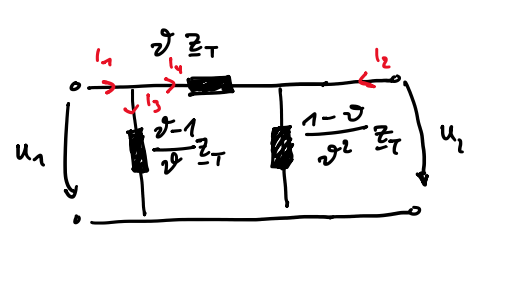
\includegraphics[width=.7\textwidth]{fundamentals/pi_transformer.png}
    \caption[$\Pi$-representative circuit of a transformer with a longitudinal tap changer]{$\Pi$-representative circuit of a transformer with a longitudinal tap changer; own figure after \autocite{machowskiPowerSystemDynamics2020,burlakinEnhancedVoltageControl2024}}
    \label{fig:pi-transformer}
\end{figure}

\begin{align}
    \underline{I}&=\underline{\mab{Y}} \cdot \underline{U} \notag \\[12pt]
    \begin{bmatrix}
        \underline{I}_1 \\
        \underline{I}_2
    \end{bmatrix}&= 
    \begin{bmatrix}
        \underline{Y}_{11} & \underline{Y}_{12} \\
        \underline{Y}_{21} & \underline{Y}_{22}
    \end{bmatrix} \cdot
    \begin{bmatrix}
        \underline{U}_1 \\
        \underline{U}_2
    \end{bmatrix} \label{eq:admittance}
\end{align}

The admittance matrix of a two port network can be expressed after \textcite{machowskiPowerSystemDynamics2020} as \autoref{eq:admittance}. For the $\Pi$-model of an \acs{OLTC} transformer it is leading to \autoref{eq:admittance-oltc}.
% \sidenote(1.7cm){$\Pi$-admittance matrix}
\begin{align}
    \underline{\mab{Y}}_\mathrm{\Pi,T}&= 
    \begin{bmatrix}
        \underline{Y}_\mathrm{T} & -\underline{\vartheta}\underline{Y}_\mathrm{T} \\
        \underline{\vartheta}^*\underline{Y}_\mathrm{T} & -\underline{\vartheta}^*\underline{\vartheta}\underline{Y}_\mathrm{T}
    \end{bmatrix} \label{eq:admittance-oltc}
\end{align}
Another way of writing down the admittance matrix is shown in \autoref{eq:admittance-oltc-2}. It is considering, that the matrix can be split up in a symmetric, constant part, and a variable current injection part. The latter is not symmetrical and depends on the tap position of the transformer. Therefore in some simulation algorithms the static part is used in the admittance matrix, and the variable part is considered in the current injection vector. \autocite{machowskiPowerSystemDynamics2020}

\begin{align}
    \begin{bmatrix}
        \underline{I}_1 \\
        -\underline{I}_2
    \end{bmatrix} &=
    \begin{bmatrix}
        \underline{Y}_\mathrm{T} & -\underline{Y}_\mathrm{T} \\
        -\underline{Y}_\mathrm{T} & \underline{Y}_\mathrm{T}
    \end{bmatrix}
    \begin{bmatrix}
        \underline{U}_1 \\
        \underline{U}_2
    \end{bmatrix} -
    \begin{bmatrix}
        \Delta \underline{I}_1 \\
        \Delta \underline{I}_2
    \end{bmatrix}\text{, where } \notag \\[12pt]
    \begin{bmatrix}
        \Delta \underline{I}_1 \\
        \Delta \underline{I}_2
    \end{bmatrix} &=
    \begin{bmatrix}
        \underline{0} & (\underline{\vartheta}-1)\underline{Y}_\mathrm{T} \\
        -(\underline{\vartheta}^*+1)\underline{Y}_\mathrm{T} & (\underline{\vartheta}^*\underline{\vartheta}+1)\underline{Y}_\mathrm{T}
    \end{bmatrix}
    \begin{bmatrix}
        \underline{U}_1 \\
        \underline{U}_2
    \end{bmatrix} \text{ leading to } \notag \\[12pt]
    \underline{\mab{Y}}_\mathrm{\Pi,T}&= 
    \begin{bmatrix}
        \underline{Y}_\mathrm{T} & -\underline{Y}_\mathrm{T} \\
        -\underline{Y}_\mathrm{T} & \underline{Y}_\mathrm{T}
    \end{bmatrix} -
    \begin{bmatrix}
        \underline{0} & (\underline{\vartheta}-1)\underline{Y}_\mathrm{T} \\
        -(\underline{\vartheta}^*+1)\underline{Y}_\mathrm{T} & (\underline{\vartheta}^*\underline{\vartheta}+1)\underline{Y}_\mathrm{T}
    \end{bmatrix} \label{eq:admittance-oltc-2}
\end{align}

\subsubsection*{Per unit system specialities}

Reactances and resistances are referred to the base voltage and apparent power of the operational unit, such as the transformer. The power system simulation uses its own base voltage and base apparent power, enabling the use of one single calculation domain. This is done to simplify the calculation and to make the results easily comparable to each other. Hence, the reffered values have to be transformed from the equipment based values to the simulation based values. The relations and conversions are defined as follows.

\begin{align}
    &\underline{Y}_\mathrm{T}=\frac{1}{r_\mathrm{T} + x_\mathrm{T} \cdot j} \cdot \frac{b_\mathrm{T} \cdot j}{2} \notag \\[12pt]
    &\underline{Y}_\mathrm{T,~sim}=\underline{Y}_\mathrm{T} \cdot \frac{S_\mathrm{n}}{S_\mathrm{n,~sim}} \label{eq:y-t-based} \\[12pt]
    &\underline{U}_\mathrm{whatever,~sim}=\underline{U}_\mathrm{whatever} \cdot \frac{S_\mathrm{n}}{S_\mathrm{n,~sim}} \label{eq:voltages-based}
\end{align}

Displayed like in \autoref{eq:y-t-based}, the characteristic of the operational unit is referred to the simulation base value. Here, the admittance of the transformer is multiplied with its own rated apparent power, then devided by the apparent power of the simulation system. Similar, the voltages are calculated via \autoref{eq:voltages-based}. This specialities are considered in the tap changer modeling, thus further information is given in \autocite{machowskiPowerSystemDynamics2020}, Appendix A.

\commenting{
    Additionally to consider:
    \begin{itemize}
        \item D-q transformations (???),
        \item Frequency domains: reactances and inductances are dependent and can change with the base frequency,
        \item Torque and power relations.
    \end{itemize}
    }

\subsection{Open-Source Power System Simulation tools}
    
\commenting{
    Some information about other open source python power system simulation tools, such as:
    \begin{itemize}
        \item Pandapower,
        \item TOPS,
        \item ... .
    \end{itemize}
    Build up like a scan (see Georg's thesis).
    
    BUT: As well including the there used implementation of transformers mathematical background and complexity.
}
        
%%%%%%%%%%%%%%%%%%%%%%%%%%%%%%%
\section{Voltage stability basics}

\subsection{Voltage stability definitions, classifications, and conditions}
A Practical introduction to voltage stability assessment, methods and indices is given in the standard and extending literature of \textcite{rueda-torresEvaluationVoltageStability2024,danishVoltageStabilityElectric2015,cutsemVoltageStabilityElectric1998}.

\commenting{
    Interesting to note/implement here: Basic classification, definitions, and the nature or conditions of voltage stability. Such as
    \begin{itemize}
        \item Short term vs. long term
        \item Static vs. dynamic
        \item Transmission driven vs. load driven vs. generation driven; stability/instability, and/or contributions 
        \item Influence OLTC: Restoring voltage level, but not adding reactive capacities; hence adding risk of voltage collapses
        \item Load vs. transmission aspects
        \item Example mechanism: \textbf{Collapse effect of the nordic test system} \autocite{vancutsemTestSystemsVoltage2020,cutsemVoltageStabilityElectric1998}
    \end{itemize}
}
        
\begin{table}
    \centering
    \caption{Voltage instability types and different time frames with examples; after \quelle}
    \small
    \renewcommand\tabularxcolumn[1]{m{#1}}
    \vspace*{12pt}
    \begin{tabularx}{\textwidth}{llXX}
        \toprule
        \textbf{No} & \textbf{Type} & \textbf{Cause of incident} & \textbf{Time frames} \\
        \toprule
        1 & Long-term & Slowly use up of reactive reserves and no outage & Several minutes to several hours \\
        2 & Classical & Key outage leads to reactive power shortage & One to five minutes \\
        3 & Short-term & Induction motor stalling leads to reactive power shortage & Five to fifteen seconds \\
        \bottomrule
    \end{tabularx}
\end{table}

\subsection{Stability Indices}

One easy idea for obtaining a stable operation is looking at the Jacobian Matrix. If this matrix is getting singular, the System will not remain in a stable operation. Singularity of matrices is checked by follwing two hypothesis tests:
\begin{align}
    &\det(\mab{J})=0 \label{eq:jacobian-det} \\[12pt]
    &J \times J^{-1} \uparrow \label{eq:jacobian-rank}
\end{align}
The Jacobian Matrix is defined as:
% \sidenote(5.2cm){Jacobian Matrix}
\begin{align}
    \mab{J}=
    \begin{bmatrix}
        \Delta \mab{P} \\
        \Delta \mab{Q}
    \end{bmatrix}&=
    \begin{bNiceArray}{c|c}
        \mab{H} & \mab{M'} \\ \hline
        \mab{N} & \mab{K'}
    \end{bNiceArray} \cdot
    \begin{bmatrix}
        \Delta \delta \\
        \Delta V/V
    \end{bmatrix} \notag \\[12pt]
    \begin{bmatrix}
        \Delta P_1 \\
        \vdots \\
        \Delta P_n \\ \hline
        \Delta Q_1 \\
        \vdots \\
        \Delta Q_n
    \end{bmatrix}&=
    \begin{bNiceArray}{ccc|ccc}
        \frac{\partial P_1}{\partial \delta_1} & \hdots & \frac{\partial P_1}{\partial \delta_n} & V_1\frac{\partial P_1}{\partial V_1} & \hdots & V_n\frac{\partial P_1}{\partial V_n} \\
        \vdots & \ddots & \vdots & \vdots & \ddots & \vdots \\
        \frac{\partial P_n}{\partial \delta_1} & \hdots & \frac{\partial P_n}{\partial \delta_n} & V_1\frac{\partial P_n}{\partial V_1} & \hdots & V_n\frac{\partial P_n}{\partial V_n} \\ \hline
        \frac{\partial Q_1}{\partial \delta_1} & \hdots & \frac{\partial Q_1}{\partial \delta_n} & V_1\frac{\partial Q_1}{\partial V_1} & \hdots & V_n\frac{\partial Q_1}{\partial V_n} \\
        \vdots & \ddots & \vdots & \vdots & \ddots & \vdots \\
        \frac{\partial Q_n}{\partial \delta_1} & \hdots & \frac{\partial Q_n}{\partial \delta_n} & V_1\frac{\partial Q_n}{\partial V_1} & \hdots & V_n\frac{\partial Q_n}{\partial V_n} \\
    \end{bNiceArray} \cdot
    \begin{bmatrix}
        \Delta \delta_1 \\
        \vdots \\
        \Delta \delta_n \\ \hline
        \Delta V_1/V_1 \\
        \vdots \\
        \Delta V_n/V_n
    \end{bmatrix}
\end{align}

Although this method seems easy to implement, there are some numerical problems realted to that. Checking if a Matrix is singular with numerical mathods, can only be realised as a probablilty expression. A result could be, that the determinant of the matrix is below a certain threshold. The algorithm would propose, that the matrix is probabilistic singular. \commenting{[QUELLE]} This problem leads to the necessity of applying other methods or indices for stability assessment. \textcite{danishVoltageStabilityElectric2015} is proposing a few other indices, that are based on the Jacobian Matrix, and shows comparitive characteristics between Jacobian Matrix and system variable based voltage stability indices. These Jacobian Matrix based indices are listed and further described in \autoref{app:jacobian-voltage-indices}, while the comparative characteristics are described in \autoref{app:jacobian-vs-system-indices}. 

\subsection{Assessment methods}
        
\subsection{Analytical stability calculation of static power systems}
        
%%%%%%%%%%%%%%%%%%%%%%%%%%%%%%%
\section{Control engineering theory}

\subsection{Commonly used on-load tap changer control}

A few basics are in the interest, understanding differences between real world beahavior, or possible ways of building up a \acs{OLTC} transformer control. This control theory difference can be limiting as well for the results and objectives compared to the actual possible control in the field.

\subsubsection{Typical presets are manually set}

The target voltage is typically set from the control room of the grid operator, coming from pre-calculated load flow analysis. This can be set hours before, or even day-ahead with the estimated loads of the grid. This value is set locally for each operating unit subsequently. The control is then operating locally and without further involvement of the grid operator. \quelle

\subsubsection{Discrete controllers are used in the field}

Typically the used controller in the field is a discrete controller, which can change tap positions under load within a time frame of around few seconds. Practical tap steps are around $2~\mathrm{\%}$ of the overall transforming ratio. The control is set up with a dead band, to avoid unnecessary tap changes. It is necessecary to note here, that this control and its mathematical caracteristics contains logical elements, blocks, and delays, which cannot be translated in a typical control theory transmission function. This leads to the missing possibility to easily obtain mathematical stability for the control of the overall considered power system. \quelle

\subsection{Dynamic voltage stability}

\commenting{
    Can I really express this as \glqq Controller theory\grqq?
}

\subsection{Bifurcations and Chaos theory control}

\commenting{
    Is this necessary or already out of scope?
    \begin{enumerate}
        \item Fuzzy Control mechanisms,
        \item Neural Networks,
        \item Bifurcations.
\end{enumerate}
}